\documentclass[10pt, compress]{beamer}

\usetheme{m}

\usepackage{booktabs}
\usepackage[scale=2]{ccicons}
\usepackage{minted}

\usepackage{graphicx} %package to manage images


\usepackage{tikz}

\usetikzlibrary{scopes}
%\documentclass[tikz, border=5pt]{standalone}
\usetikzlibrary{calc}
\usetikzlibrary{patterns}
\usepackage{tkz-euclide}
\usetkzobj{all}

\usemintedstyle{trac}

\usefonttheme[onlymath]{serif}

\newcommand\der{{\rm d}}

\title{Robot Inverse Kinematics using SQP method}
\subtitle{}
\date{\today}
\author{Xiaoqian Mu, Yuechuan Xue}
\institute{Iowa State University}

\begin{document}

\maketitle

\begin{frame}[fragile]{Problem Formulation}
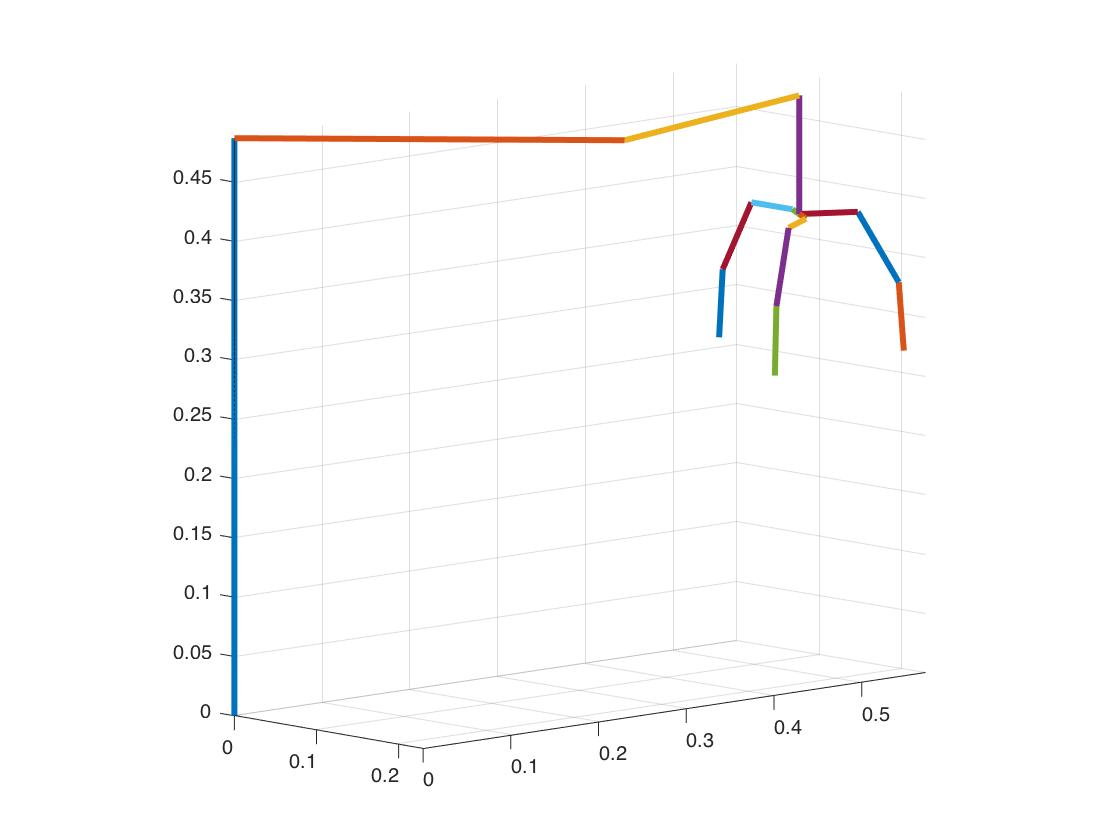
\includegraphics[width=6cm, height=4cm]{robot-matlab-config.jpg}
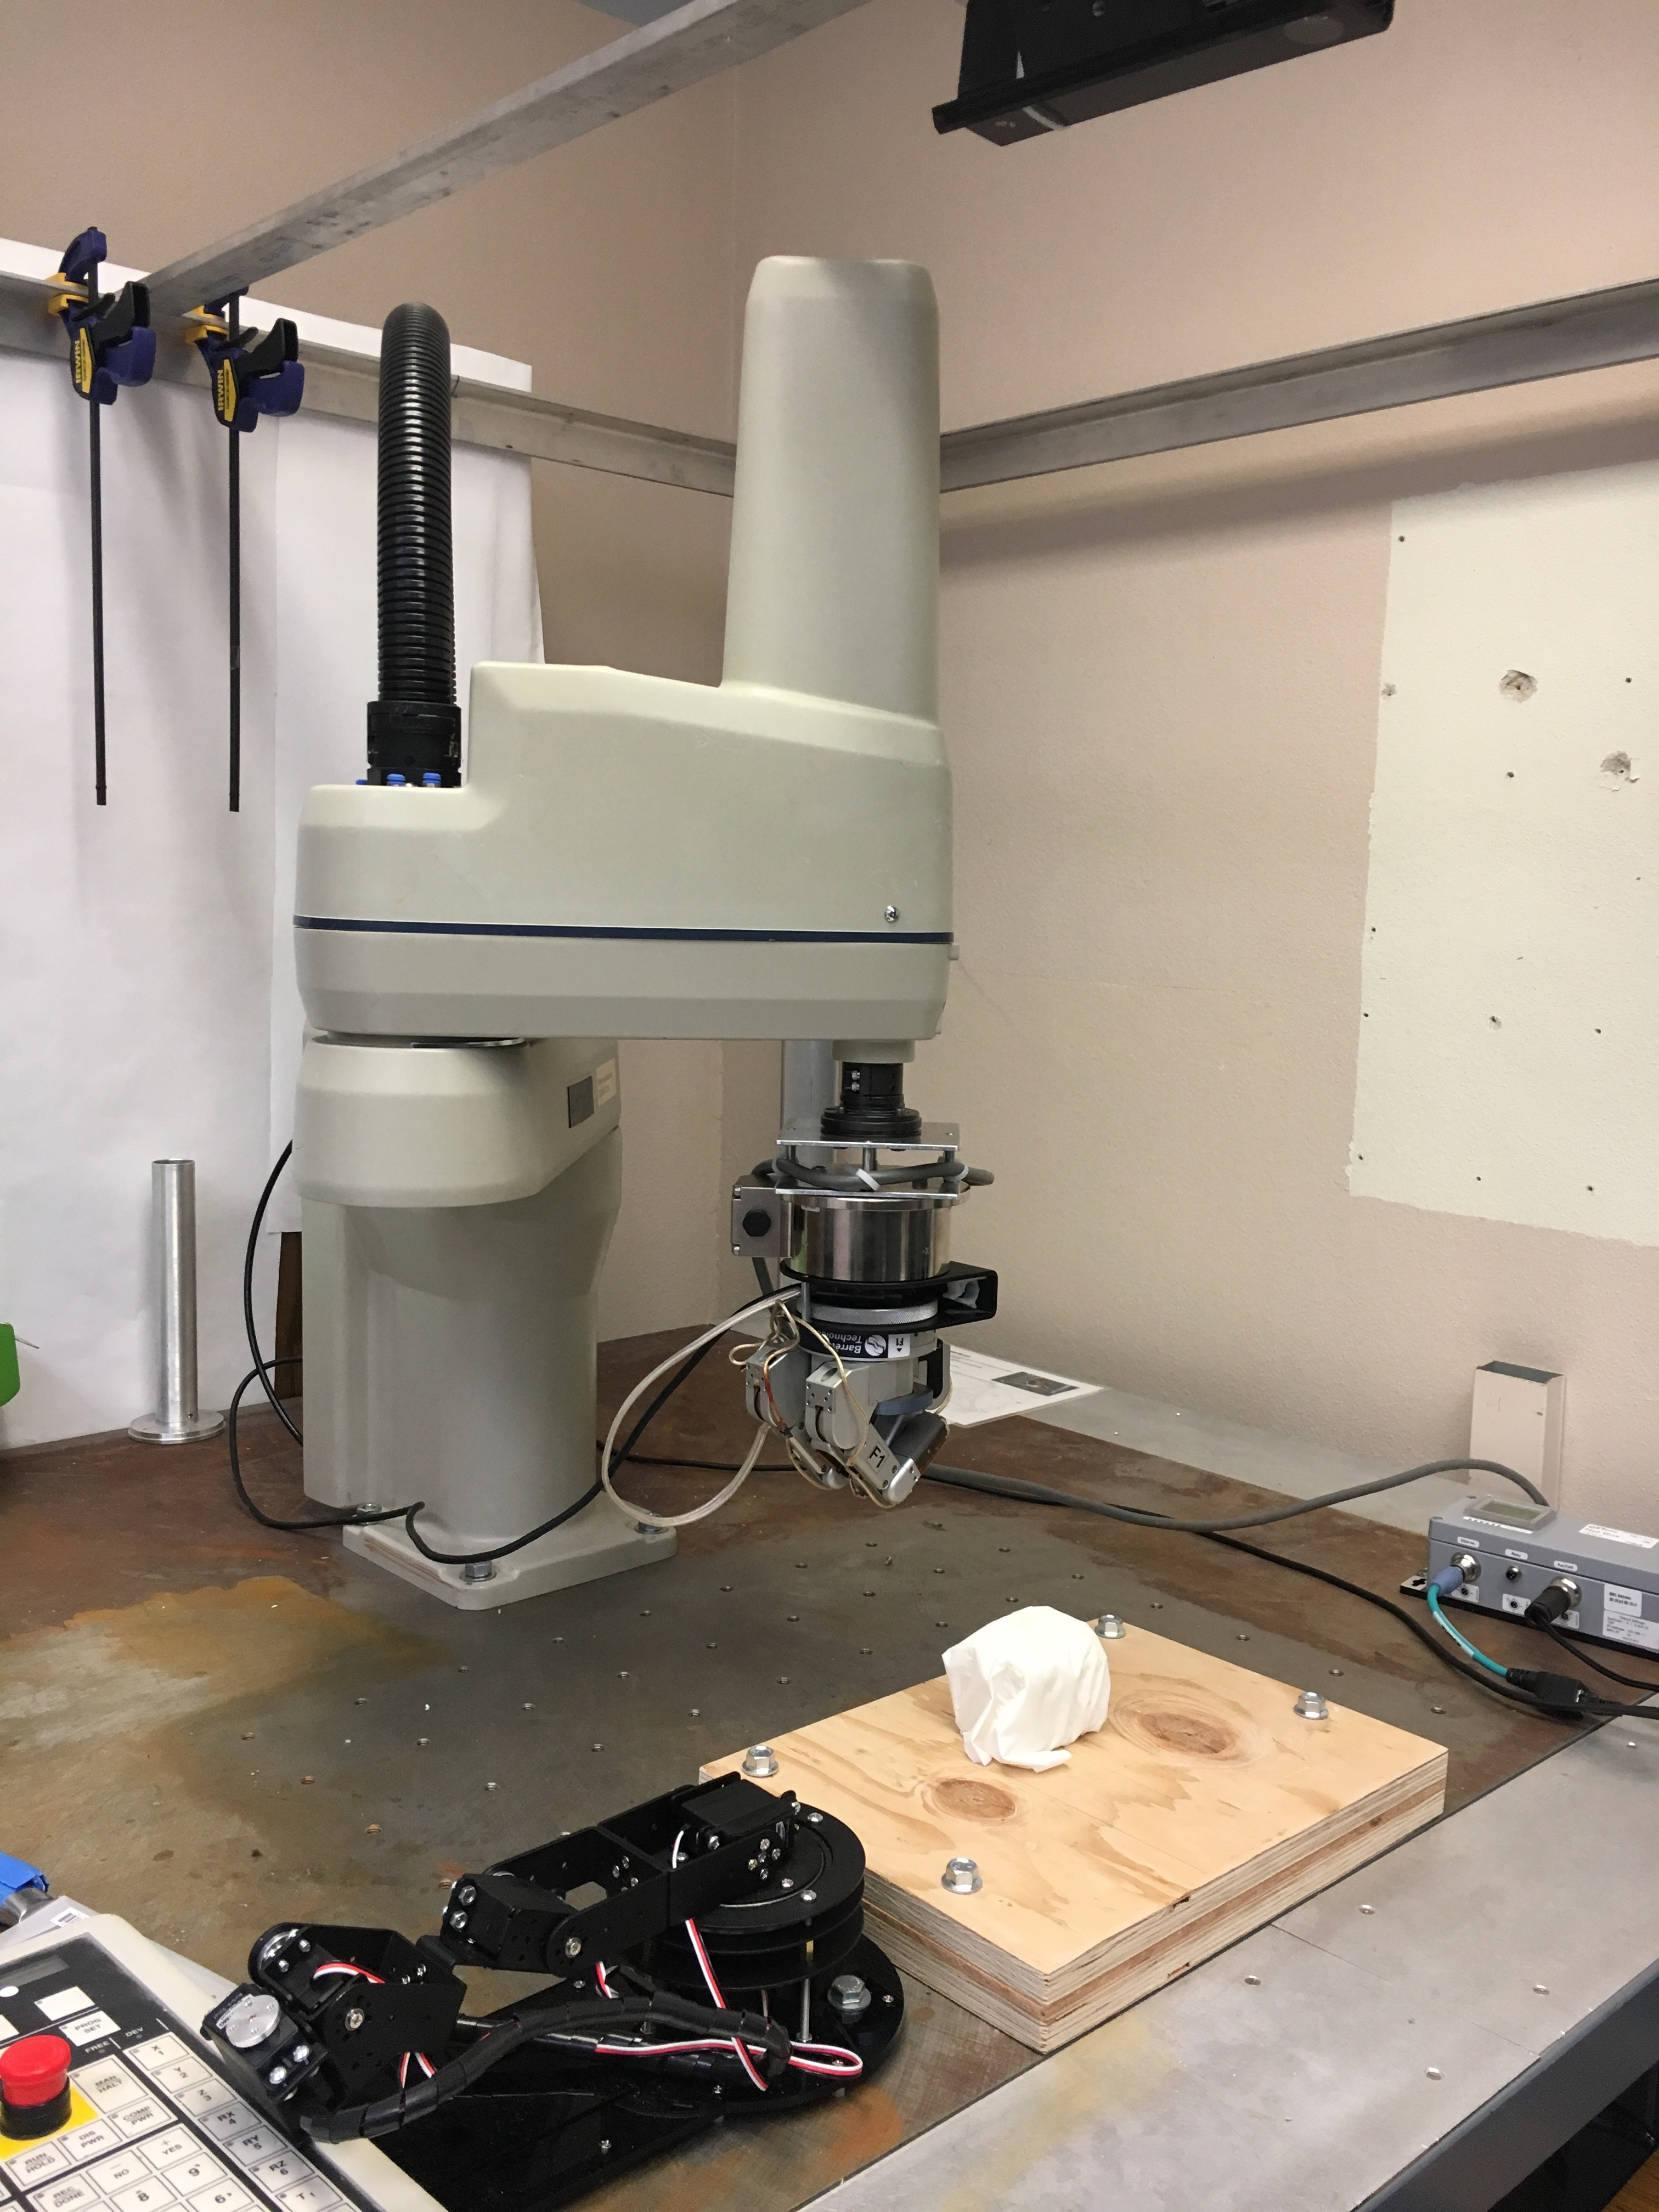
\includegraphics[width=4cm, height=5cm]{IMG_5860.jpg}
\end{frame}



\begin{frame}[fragile]{Introduction}
\begin{columns}
\begin{column}{0.5\textwidth}
In constrained optimization, the general aim is to transform the problem into an easier subproblem that can then be solved and used as the basis of an iterative process.

\vspace{0.1in}

Some early methods translate the constrained problem to a basic unconstrained problem by using a \textbf{penalty function} for constraints  that are near or beyond the constraint boundary. (Interior Point Method)
\end{column}
\begin{column}{0.5\textwidth}  %%<--- here
    \begin{center}
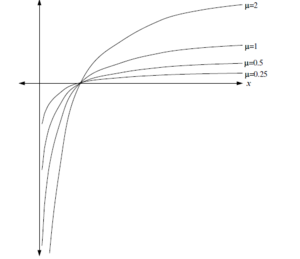
\includegraphics[width=4cm, height=5cm]{interior-point-method.png}
     \end{center}
\end{column}
\end{columns}
\end{frame}

\begin{frame}[fragile]{Introduction}
These methods are now considered relatively inefficient and have been replaced by methods that have focused on the solution of the KKT equations.

The KKT are necessary conditions for optimality for a constrained optimization problem. It is both necessary and sufficient for a global optimal point in a convex programming problem. 
\end{frame}

\begin{frame}[fragile]{Sequential Quadratic Programming}
A series of algorithms attempt to compute the Lagrange multipliers directly.

Constrained quasi-Newton methods guarantee super-linear convergence by accumulating second-order information regarding the KKT equations using a quasi-Newton updating procedure.

A quadratic programming (QP) problem will be solved at each major iteration.
\end{frame}

\end{document}